\documentclass[11pt,a4paper]{article}
\usepackage[spanish]{babel}
\usepackage[utf8]{inputenc}
\usepackage[top=2cm, bottom=2cm, left=2cm, right=2cm]{geometry}
\usepackage{commath,amsmath,lastpage,float,sectsty,hyperref,graphicx,pdfpages,fancyhdr,listings,siunitx}

\sectionfont{\fontsize{12}{15}\selectfont}
\linespread{1.25} % Interlineado 1.5
\renewcommand{\rmdefault}{phv} % Arial
\renewcommand{\sfdefault}{phv} % Arial

\hypersetup{
    pdftitle={Trabajo Práctico 1},
	pdfsubject={Análisis Numérico I},
	pdfauthor={del Mazo Federico, Kristal Juan Ignacio},
}

\lstset{
  basicstyle=\ttfamily,
  columns=fullflexible,
  frame=single,
  breaklines=true,
  postbreak=\mbox{\textcolor{red}{$\hookrightarrow$}\space},
}

\fancypagestyle{enunciado}{
    \fancyhf{}
    \fancyhead[C]{Enunciado provisto por la catedra}
}

\pagestyle{fancy}
\fancyhf{}
\fancyhead[R]{Trabajo Práctico 1 - 2018c2}
\fancyhead[L]{75.12 Análisis Numérico I}
\renewcommand{\headrulewidth}{0.4pt}
\fancyfoot[L]{100029 - 99779}
\fancyfoot[R]{\thepage de \pageref*{LastPage}}
\renewcommand{\footrulewidth}{0.4pt}
\setlength{\footskip}{17pt}

\fancypagestyle{onlyheader}{
\fancyfoot{}
}

\begin{document}

\begin{titlepage}
	\hfill
\includegraphics[width=6cm]{figuras/fiuba.jpg}
    \begin{center}
    \vfill
    \Huge \textbf{Trabajo Práctico 1}
    \vskip2cm
    \Large [75.12] Análisis Numérico I\\
    Segundo cuatrimestre de 2018
    \vfill
    \begin{tabular}{|l|c|r|}
	\hline
	Alumno & Padrón & Mail\\
	\hline
	\hline
	del Mazo, Federico & 100029 & delmazofederico@gmail.com\\
	\hline
	Kristal, Juan Ignacio & 99779 & kristaljuanignacio@gmail.com\\
	\hline
	\end{tabular}
    \vskip2cm
    \end{center}

    Curso 07:

    \begin{itemize}
    \item Dr Daniel Fabian Rodriguez
    \item Valeria Machiunas
    \item Federico Balzarotti
    \item Michael Portocarrero
    \end{itemize}

\end{titlepage}

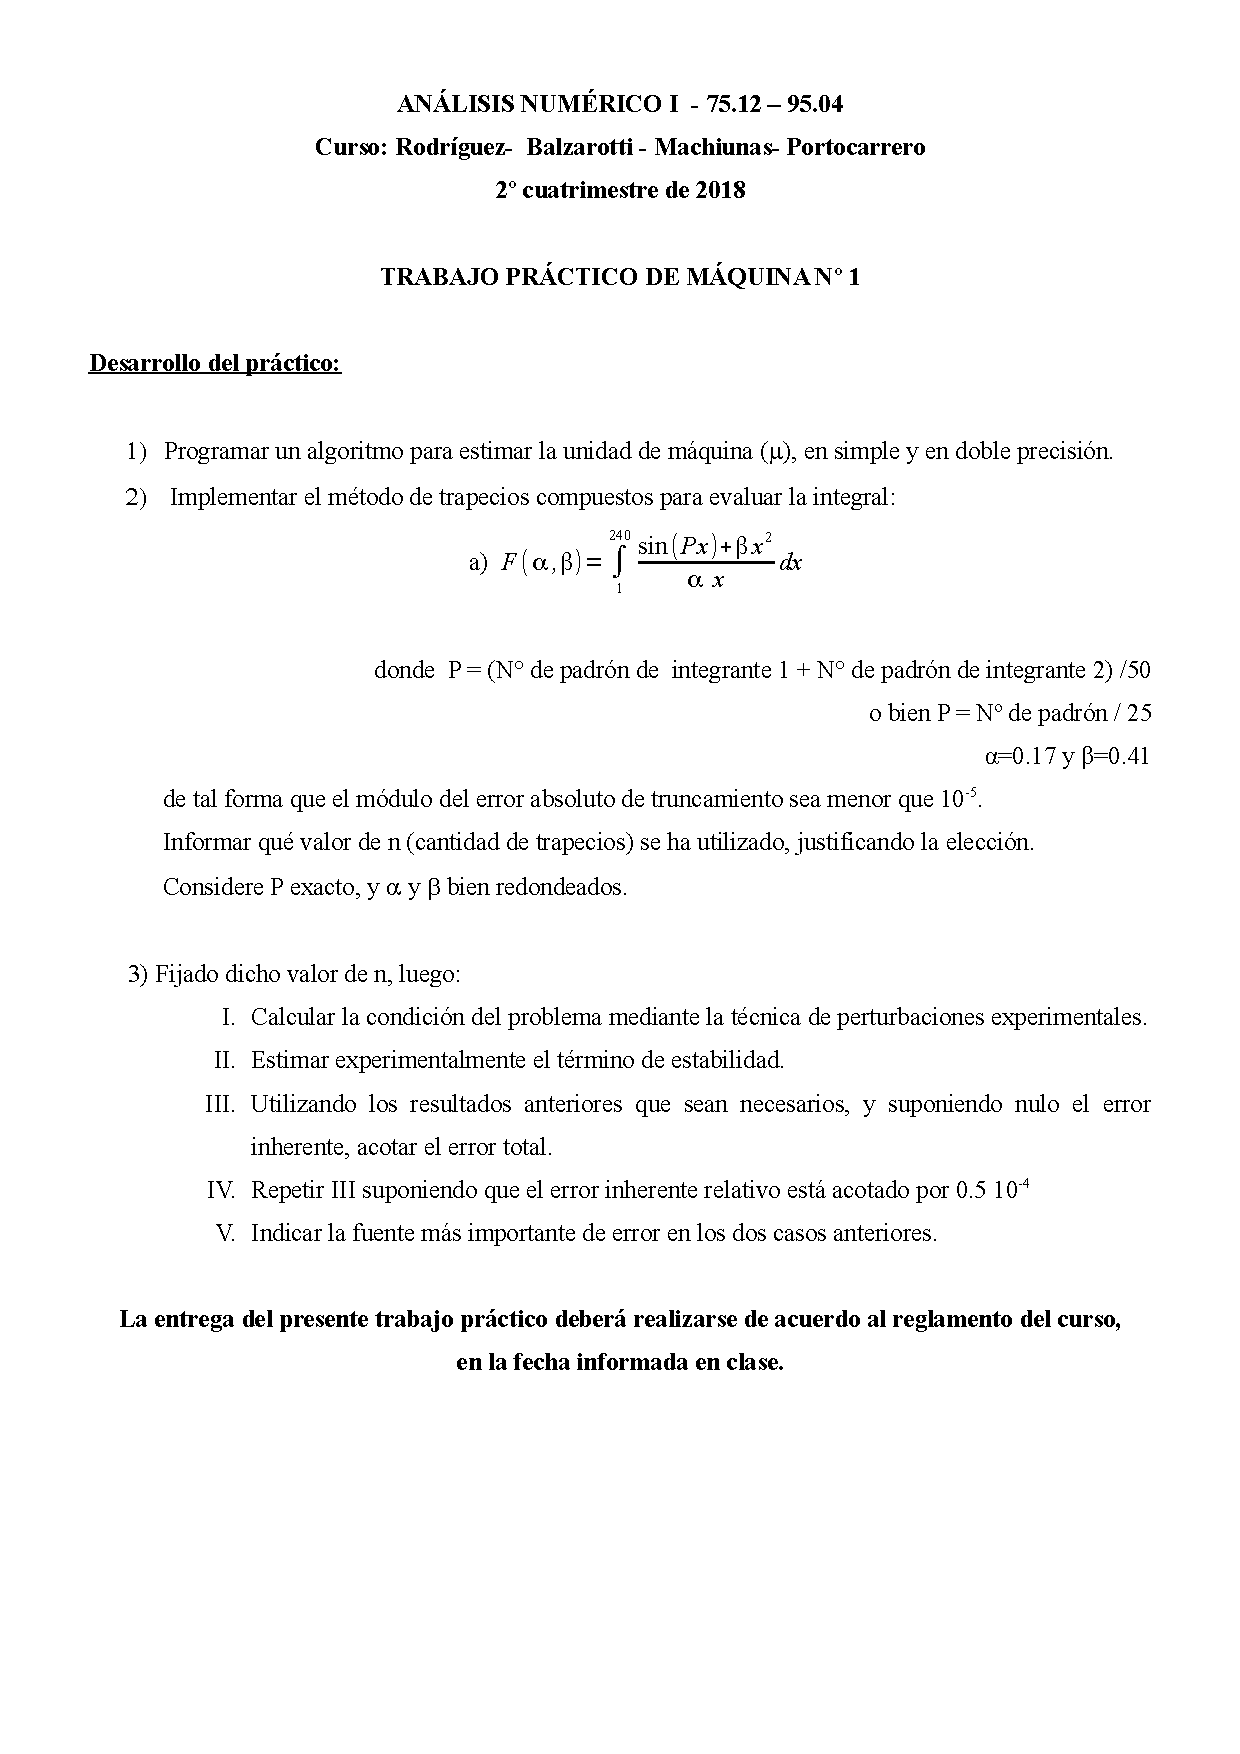
\includepdf[pages=-,pagecommand={\thispagestyle{enunciado}}]{TP1-Enunciado.pdf}

\pagenumbering{gobble}
\tableofcontents
\thispagestyle{onlyheader}
\newpage


\pagenumbering{arabic}
\setcounter{page}{1}

\section{Introducción}
El trabajo práctico tiene como objetivo el cálculo y acotamiento de errores de la siguiente integral:

\[ F(\alpha,\beta) = \int_{1}^{240}  \frac{\sin{(P x)}  + \beta x^2}{\alpha x} dx \]

Siendo:
\begin{itemize}
\item \( P = \frac{\sum\limits_{padrones}^{}}{50} = \frac{99779 + 100029}{50} = 3996.16 \) exacto 
\item \( \alpha = 0.17 \) bien redondeando
\item \( \beta = 0.41 \) bien redondeando
\end{itemize}

Específicamente:

\begin{itemize}
\item Se estimará el valor de la unidad de maquina \( \mu \).
\item Se evaluará la integral con el método de trapecios compuestos teniendo con objetivo en mente que el error absoluto de truncamiento sea menor a \num{1e-5}.
\item Se calculará computacionalmente la cantidad de trapecios utilizada en el método descrito anteriormente.
\item Se calculará la condición del problema mediante perturbaciones experimentales.
\item Se estimará experimentalmente el término de estabilidad.
\item Se acotará el error total.
\end{itemize}

\section{Desarrollo}

\subsection{Estimación de \( \mu \) }

Para los cálculos del \( \mu \) se utilizó el algoritmo del ejemplo 6.4 del libro de Hernan Gonzales \cite{Gonzales}.

\subsection{Función y sus derivadas}

Siempre teniendo en cuenta los valores de \(P, \alpha, \beta \) previamente utilizados, definimos la funcion \( f(x) \) como:

\[ f(x) = \frac{\sin{(P x)}  + \beta x^2}{\alpha x} dx \]

Graficamos la función para saber un poco más de ella en la figura \ref{fig:funcion}

\begin{figure}[H]
	\makebox[\textwidth][c]{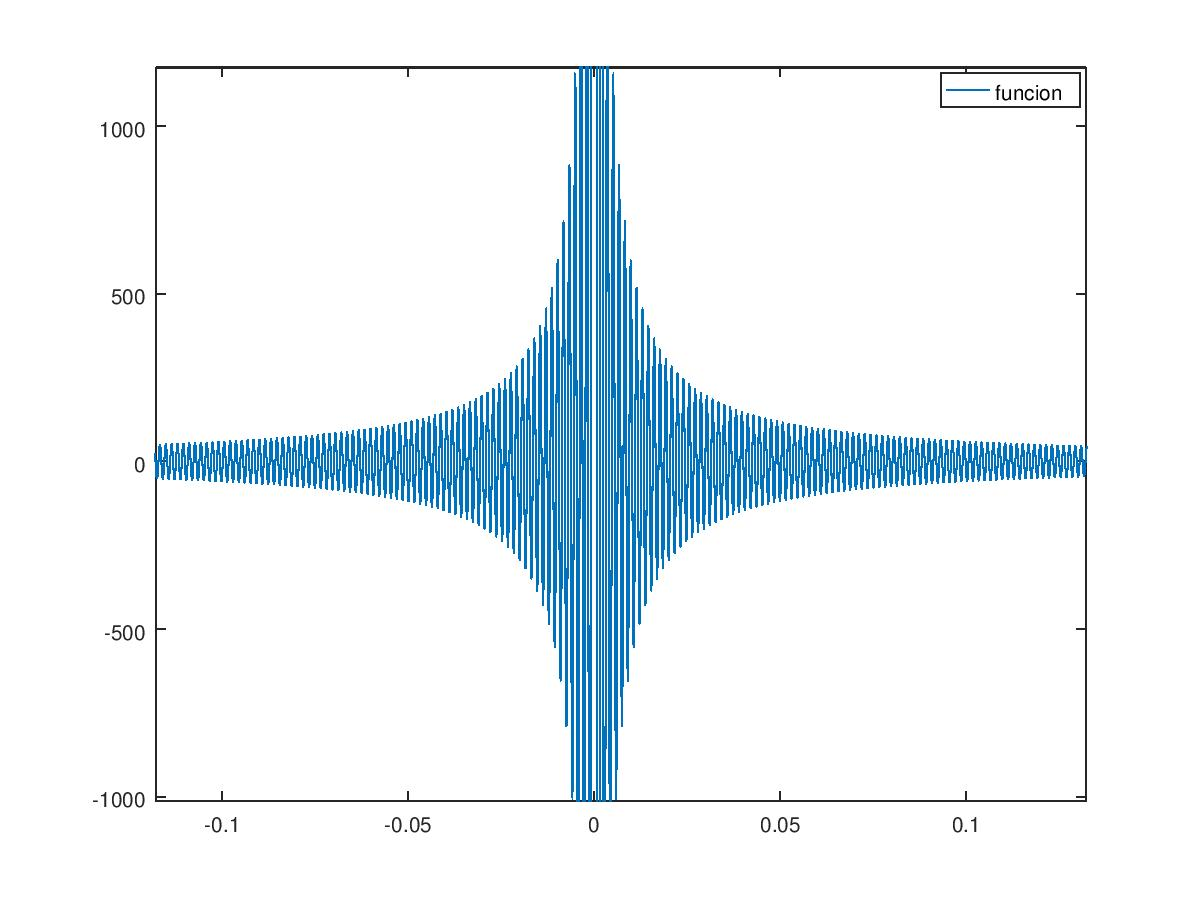
\includegraphics[width=1.2\textwidth]{figuras/funcion.jpg}}
	\caption{\(f(x)\)}
	\label{fig:funcion}
\end{figure}

De esta función calculamos sus derivadas y las graficamos en las figuras \ref{fig:funcionderivada} y \ref{fig:funcionderivada2}, para utilizar en cálculos posteriores.

\[ f'(x) = \frac{P \cos{(P x)}}{\alpha x} - \frac{ \sin{(P x)}}{\alpha x^2} + \frac{\beta}{\alpha} \]

\begin{figure}[H]
	\makebox[\textwidth][c]{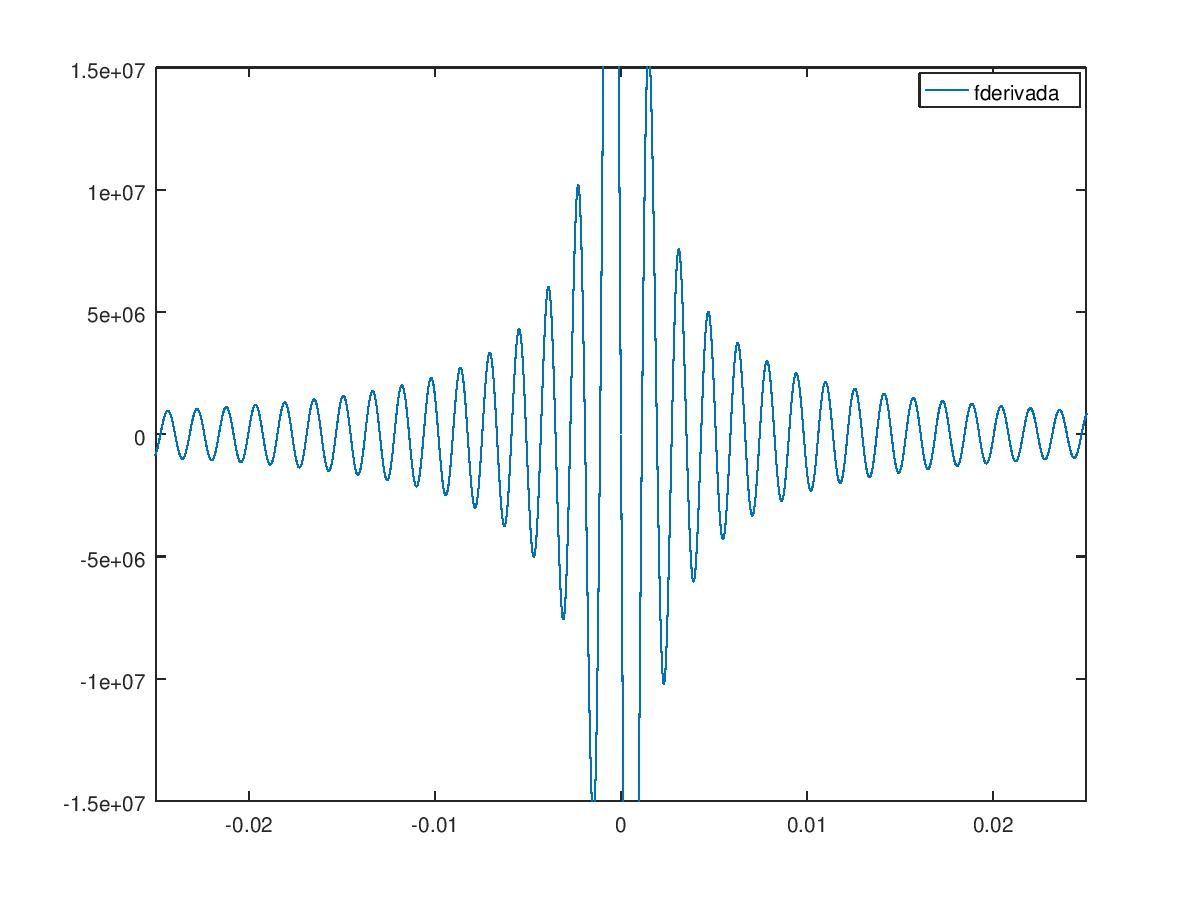
\includegraphics[width=1.2\textwidth]{figuras/funcionderivada.jpg}}
	\caption{\(f'(x)\)}
	\label{fig:funcionderivada}
\end{figure}

\[ f''(x) = - \frac{2 P \cos{(P x)}}{\alpha x^2} + \frac{2 \sin{(P x)}}{\alpha x^3} - \frac{P^2 \sin{(P x)}}{\alpha x}\]

\begin{figure}[H]
	\makebox[\textwidth][c]{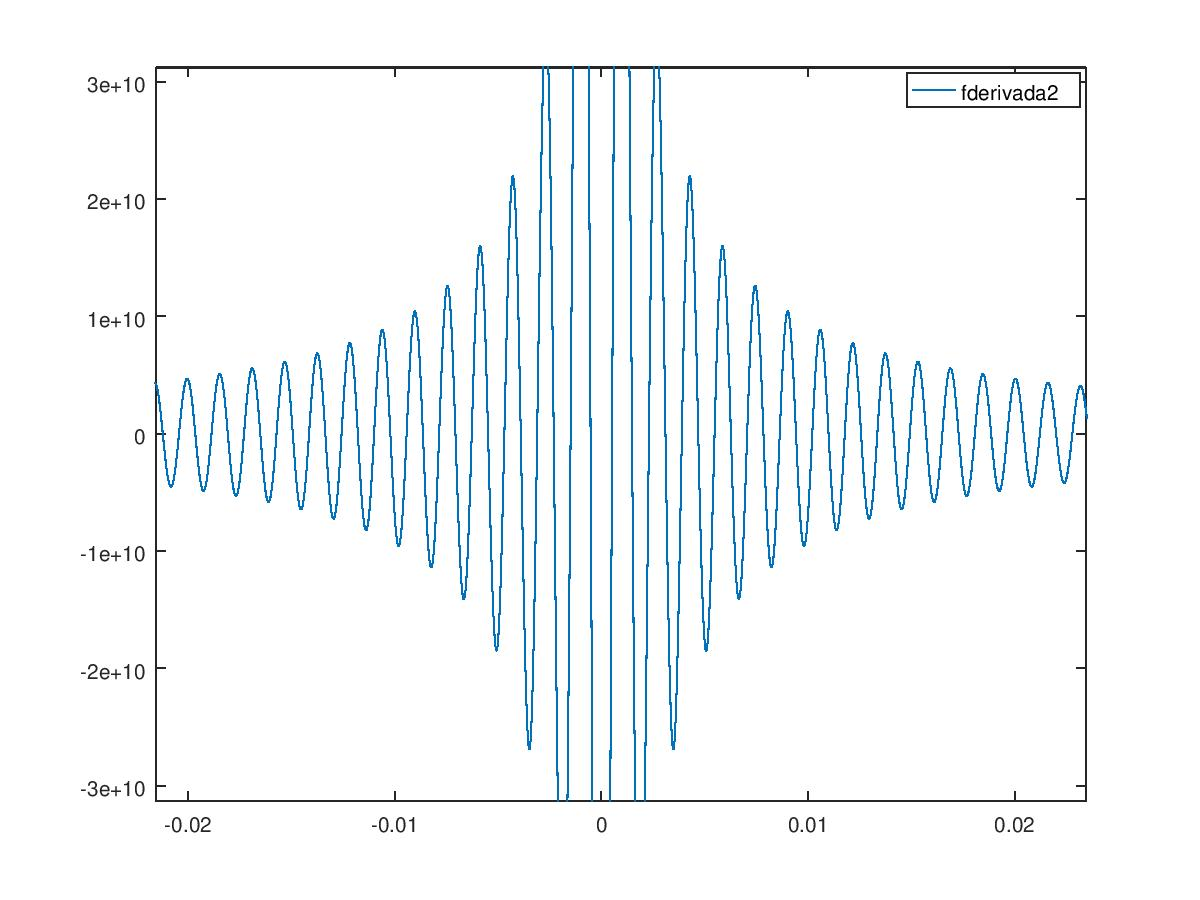
\includegraphics[width=1.2\textwidth]{figuras/funcionderivada2.jpg}}
	\caption{\(f''(x)\)}
	\label{fig:funcionderivada2}
\end{figure}

\subsection{Método de trapecios compuestos}

Sabemos que el error de truncamiento producido por el método de trapecios compuestos es:

\[ \epsilon_t = - \frac{{(b - a)}^3}{12 n^2} * f''(\xi) \]

Donde \(b, a\) son los limites de integración y \(n\) es la cantidad de trapecios. Como lo que queremos es acotar el error de truncamiento, debemos evaluar a la segunda derivada en su imagen máxima, es decir \(\xi = 1 \)

Por lo tanto, y ahora con el error de truncamiento al que queremos llegar, despejamos la cantidad de trapecios:

\[ n = \sqrt{ \abs{ - \frac{(b - a)^3 * f''(1)}{12 \epsilon_t}}} \]

\subsection{Condición del problema y término de estabilidad}


\section{Resultados}

\section{Conclusiones}

\newpage
\appendix
\section{Anexo I: Código Fuente}

\lstinputlisting[language=Octave,title=\texttt{mu.m}]{src/mu.m}

\newpage
\lstinputlisting[language=Octave,title=\texttt{main.m}]{src/main.m}

\newpage
\section{Anexo II: Resultados Numéricos}
\begin{lstlisting}[language=Octave,title=Resultados de \texttt{mu.m}]
>> mu
mu_simple =    1.0000e-08
mu_doble =    1.0000e-16
\end{lstlisting}


\begin{lstlisting}[language=Octave,title=Resultados de \texttt{main.m}]
>> main
n =    2.4160e+08
\end{lstlisting}


\newpage

\phantomsection 
\addcontentsline{toc}{section}{Bibliografía}
\renewcommand\refname{Bibliografía}
\begin{thebibliography}{9}

\bibitem{Gonzales} 
Gonzales, Hernan: 
\textit{Análisis Numérico, Primer Curso}
Buenos Aires: Nueva Librería, 2002.

\end{thebibliography}
\end{document}

